\documentclass[10pt,draftclsnofoot,onecolumn,journal,compsoc]{IEEEtran}


\setlength{\parindent}{0em}
\setlength{\parskip}{1em}



\usepackage[margin=0.75in]{geometry}
\geometry{textheight=9.5in, textwidth=7in}
\usepackage{listings}
\usepackage{comment}
\usepackage{imakeidx}
\usepackage{graphicx}
\usepackage{float}
\usepackage{listings}
\usepackage{url}
\usepackage{caption}
\usepackage{geometry}
\usepackage{enumitem}
\usepackage{setspace}
\singlespacing


\def \DocType{		%Problem Statement
	%Requirements Document
	%Technology Review
	Design Document
	%Progress Report
}



\lstset{
  basicstyle=\small\ttfamily,
 numbers=left,
  numberstyle=\scriptsize,
  showspaces=false,
  showstringspaces=false,
  breaklines=true
}





% 1. Fill in these details
\def \CapstoneTeamName{DSCVL-Overcomers}
\def \CapstoneTeamNumber{69}
\def \GroupMemberOne{KIN-HO LAM}
\def \GroupMemberTwo{LUCIEN-ARMAND T. TAMNO}
\def \CapstoneProjectName{Depth Sensing using Computer Vision and Lydar}
\def \CapstoneSponsorCompany{}
\def \CapstoneSponsorPerson{ D. Kevin McGrath}

\usepackage{datetime}
\newdate{date}{26}{3}{2018}
\date{\displaydate{date}}

\title{\centering
			
\includegraphics[height=4cm,natwidth=200,natheight=300]{images/osu_logo.eps}\\\vspace{.5in}
		\scshape{\huge CS CAPSTONE \DocType \\\vspace{.5in}
		\textbf{\Huge\CapstoneProjectName}\\\vspace{1in}
		\large	\displaydate{date}\\\vspace{.2in}		
			\large {Prepared For}\\\vspace{.1in}
			\textbf{{\Large \CapstoneSponsorPerson}} \\\vspace{.8in}		
				\large {By} \\\vspace{.1in}
				\textbf {Group \CapstoneTeamNumber}\\\vspace{.1in}
				\Large {\CapstoneTeamName}\\\vspace{.1in}
				\textbf{ { \GroupMemberTwo}}
}  
}

\IEEEtitleabstractindextext{

 \begin{abstract}
   The  Depth sensing with computer vision and lidar project ultimate goal is to deliver new kinds of images by painting an existing overlaid lidar scanner point-cloud against over a camera image. When completed, the comprehensive python program will allow use-defined information through the user-friendly interface to display a single output image from two different technologies . Thus, this document is written to provide details about the depth sensing with computer vision and lidar  software design descriptions.     
 
 \end{abstract} 
 

}

\begin{document}
\pagenumbering{gobble}
 \maketitle
\IEEEdisplaynontitleabstractindextext
\IEEEpeerreviewmaketitle
\newpage
\pagenumbering{arabic}
\tableofcontents
\newpage

\section{Overview}
As a roadmap, this document is to help its users understand how to build accurate overlay images from two existing, reliable technologies with distinctive features. The Lidar technology description would help the reader to understand how accurate and reliable are the pulsing laser distance measurements in this outdoor environment while the Webcam would aide to get the two-dimensional image to overlay to the depth Lidar scanner sensor data inputs.
\subsection{Scope}
This document is to describe a new application that will combine both the Lidar technology to Webcam stream technology for specific overlay images to define accurate objects distances in outdoor environment to be utilized by the stakeholders  and specially client of the DSCVL project.

\subsection{Purpose}
The purpose of this document is to elaborate on technical aspects of the software to implement, to allow stakeholders of DSCVL project to understand what the Lidar and camera  technologies do the best, each technology characteristics,their differences and what is used to make these technologies work together in order to accomplish the ultimate goal that is to get an overlay image as required by the client.Thus, the technicality of the project different compounds would be described with great details  in the following sections. 

\subsection{Intended Audience}
 The content of this document is to primarily address the needs and requirements of the depth sensing using with computer vision client in particular and can be added more broadly, stakeholders  and even generally readers with interest on this descriptive document.
\section{Definitions}


		\textbf{IR: }\label{def:IR}
		IR refers to the infrared light spectrum.

		\textbf{IR Depth Sensor: }\label{def:depthsensor}
		A device that calculates distances by emitting infrared patterns. 
		
		\textbf{LIDAR: }\label{def:lidar}
		Light Detection And Ranging - A method that uses lasers to measure distance
		
		\textbf{Microsoft Kinect: }\label{def:kinect}
		A product that uses an IR Depth sensor to measure distances.
		
		\textbf{Logitech Brio Webcam: }\label{def:brio}
		The webcam model this project shall be using.
		
		\textbf{RPLidar A1: }\label{def:rplidar}
		A low-cost LIDAR unit that this project shall be using.
		
		\textbf{RPLidar Solid-state: }\textbf{RPLidar: }\label{def:rplidar2}
		A High-cost LIDAR unit single direction with better performances of detecting, measuring and locating liquids and people
		
		\textbf{Computer Vision: }\label{def:vision}
		The methods for acquiring, processing, analyzing, and classifying digital images and extracting information.
		
		\textbf{GUI: }\label{def:gui}
		GUI: Graphical User Interface
		
		\textbf{Videocapture: }\label{def:videocapture}
		videocapture: Stream of subsequent images
		
		\textbf{DSCVL: }\label{def:DSCVL}
		Acronym that stands for Depth sensing with computer vision and lidar
		
		\textbf{SDD: }\label{def:SDD}
		software design descriptions as defined by the IEEE 1016

\section{Design Description Information}
 
	\subsection{Introduction}
	The design description information presents to the reader what kinds of information the DSCVL processes, what part of the Lidar or the camera technology handles what and how.
    
    \subsection{Design Description Identification}
   Essentially,there are two blocks or components that are ought to interact  to make the Depth sensing using computer vision become a feasible project, and those two components are the hardware and the software. The hardware uses the robopeak lidar A1 scanner and the Logitech Brio webcam of which, we provide more details after. The software component basically having a bunch of open source libraries among others the OpenCV library, the Numpy library and others.  
    	\subsubsection{Object processing At the hardware level}
    	\paragraph{\textbf {Robopeak Lidar or RPLidar Inputs}} 	
    	We use the RPLidar as input device to our system to provide accurate measurements of distances via its sensors. In detecting, locating and measuring objects that include people and liquids, the Lidar's scanner challenges the limits imposed by the same objects to other technologies such as the commercial infrared technology that uses  depth sensors in a natural outdoor environment but is confused by the sunlight. However, as depicted by the figure1 underneath, the most effective RPLidar model to use would be the solid-state, for it has no additional time caused by the spinning engine rotation as seen in the 360 RPLidar A1 model.
    	\\[2ex]
    	\begin{figure}[ht]
    	 \centering 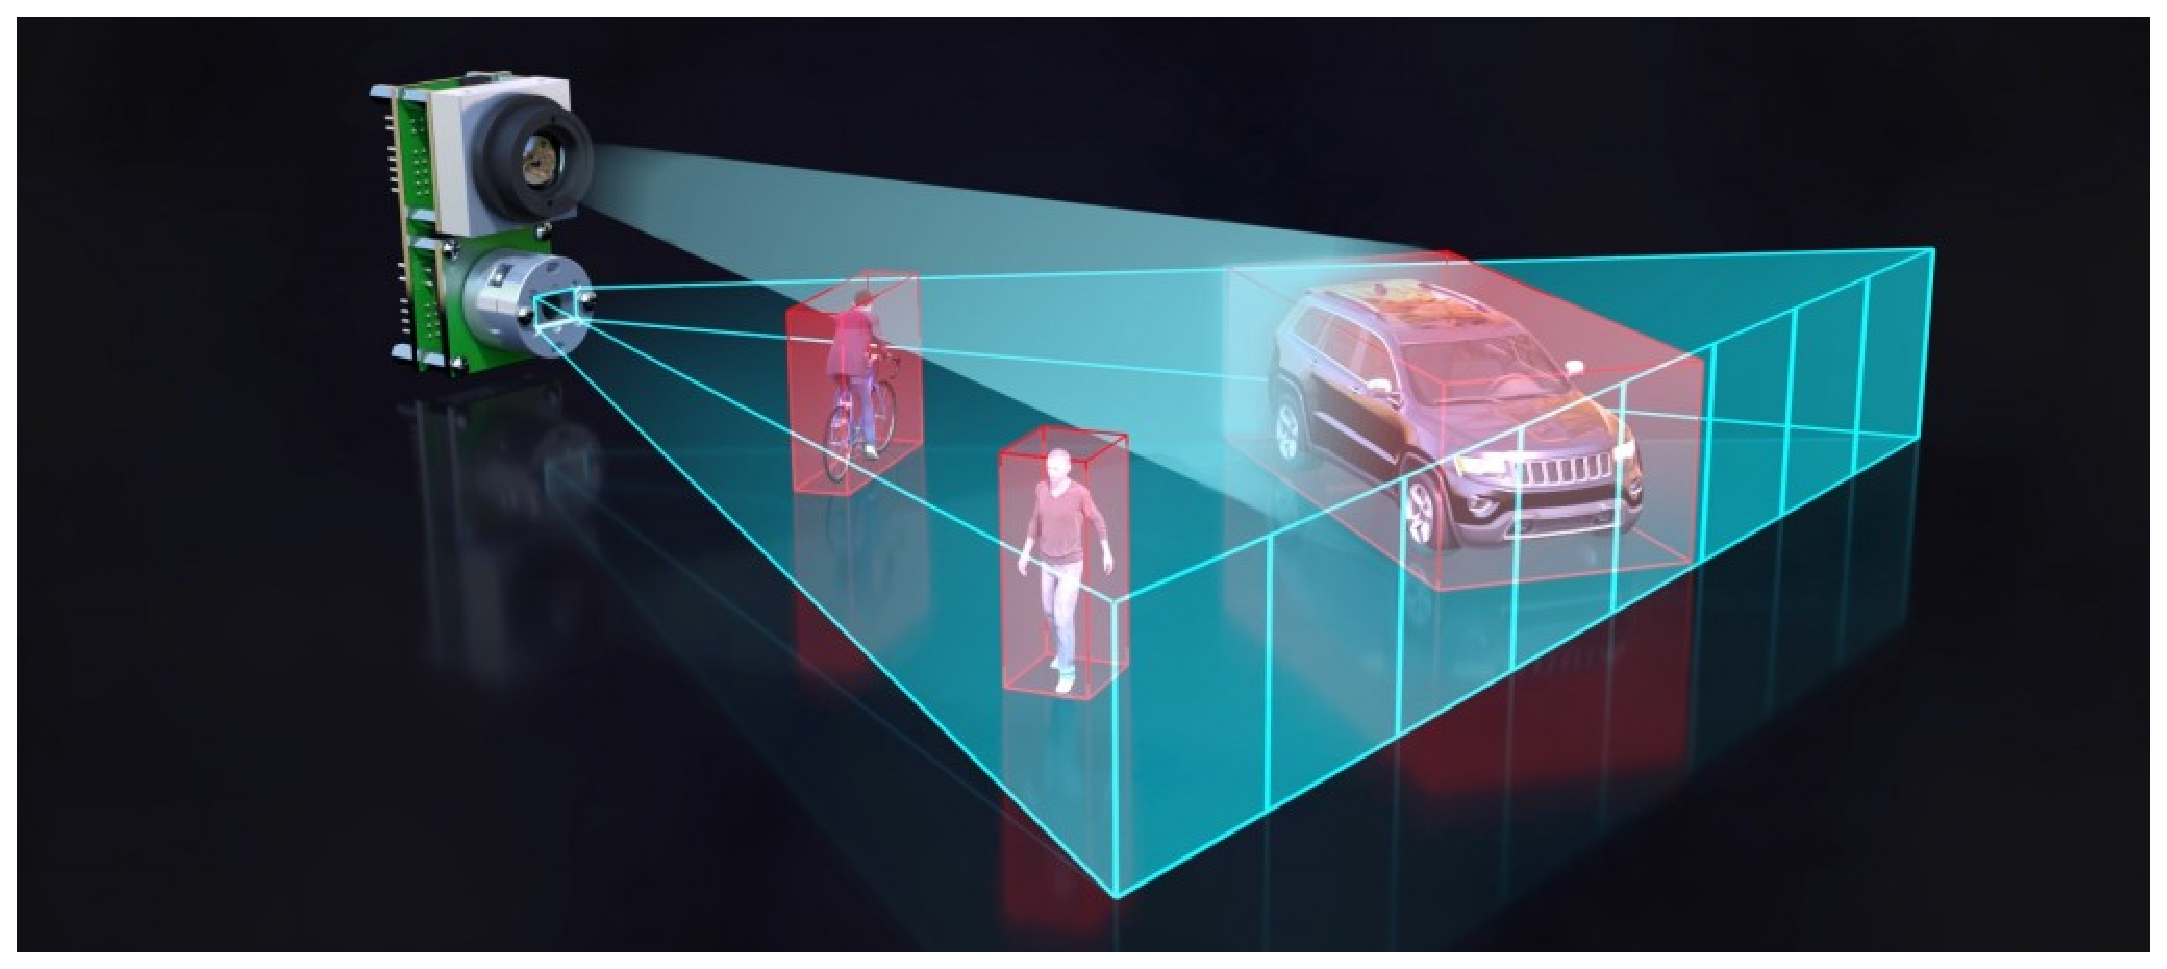
\includegraphics[width=4.5in,natwidth=4000,natheight=200]{images/LiDAR-fundamentals-2-1024x449.eps}
    	\captionof{figure}{LIDAR SENSOR FUNDAMENTALS, derived from  \textit{leddartech} }[1]\label{rplidar2}
    	\end{figure}
    	\paragraph{\textbf{The Webcam Inputs} }
    The camera is the other input device source that we will use to get video streams to match to the RPLidar sensors laser pulses, that enables us to  see what kin of object the system is processing. And both Lidar scanner and the webcam having their data process at the software level.
   
    	\subsubsection{Object processing At the software level}
    	what we are using at the software level is a array of libraries and most are python library dealing with images. we have for instance, the OpenCV library through which images found in the system would be isolated from the stream of images, processed and ultimately painted on a screen.
    	
    	\subsubsection{Library Structure}
    	The library structure aims to integrate different software functions and defines the path to the final overlay image implementation.In technical terms, the library structure is known by the name API.
    	
    \subsection{Identified design stakeholders}
  The depth sensing using computer vision and Lidar project stakeholders are  users interested by what the Lidar technology combines to the webcam image processing can accomplish in either production or experimental environment.   
    
    	\subsubsection{Image Data processing}
    The image data processing has to comply with user predefined conditions and take into account physics and mathematics parameters to yield excepted outcomes as  shown by the following figure for which a scanner rplidar A1 sensors mapping  is capturing targeted point object.
     \\[2ex]
    	\begin{figure}[ht]
    	 \centering 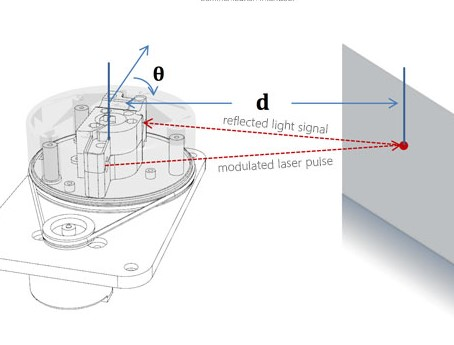
\includegraphics[width=4.5in,natwidth=4000,natheight=200]{images/imageproc.jpg}
    	\captionof{figure}{, derived from  \textit{seeeds} }[2]\label{rplidar}
    	\end{figure}
       
    	\subsubsection{the principal stakeholder}
   When it comes to the question to know who is the principal stakeholder of this python-based project, the response goes without saying that our client is D. Kevin McGrath, who has the property right on the future final DSCVL product  and therefore, all the project specifications have to meet his requirements. 
    	\subsubsection{the other stakeholders}
    	May fall into the category, users of the Lidar technology to either import new features in  production environments or those who would likely get the outcomes from the DSCVL software. 
    	
\section{Selected Design Viewpoints}
The selection of design viewpoints aims to define and present how the new system  would likely interact with its environment, address concerns from its users,choose the language to use as well as depict relations between parts.  
	\subsection{Interface viewpoint}
The virtual visible interface would be the user interface that accounts for what kinds of information a user would like to see displayed as the output.Basically, the user would like to have an overlay images in a range within the value defined on the user interface.  
That said and regardless the OS that hosts the DSCVL application, the user interface has to be standardized across platforms and its components interaction process as shown in the following figure.
\\[2ex]
    	\begin{figure}[ht]
    	 \centering 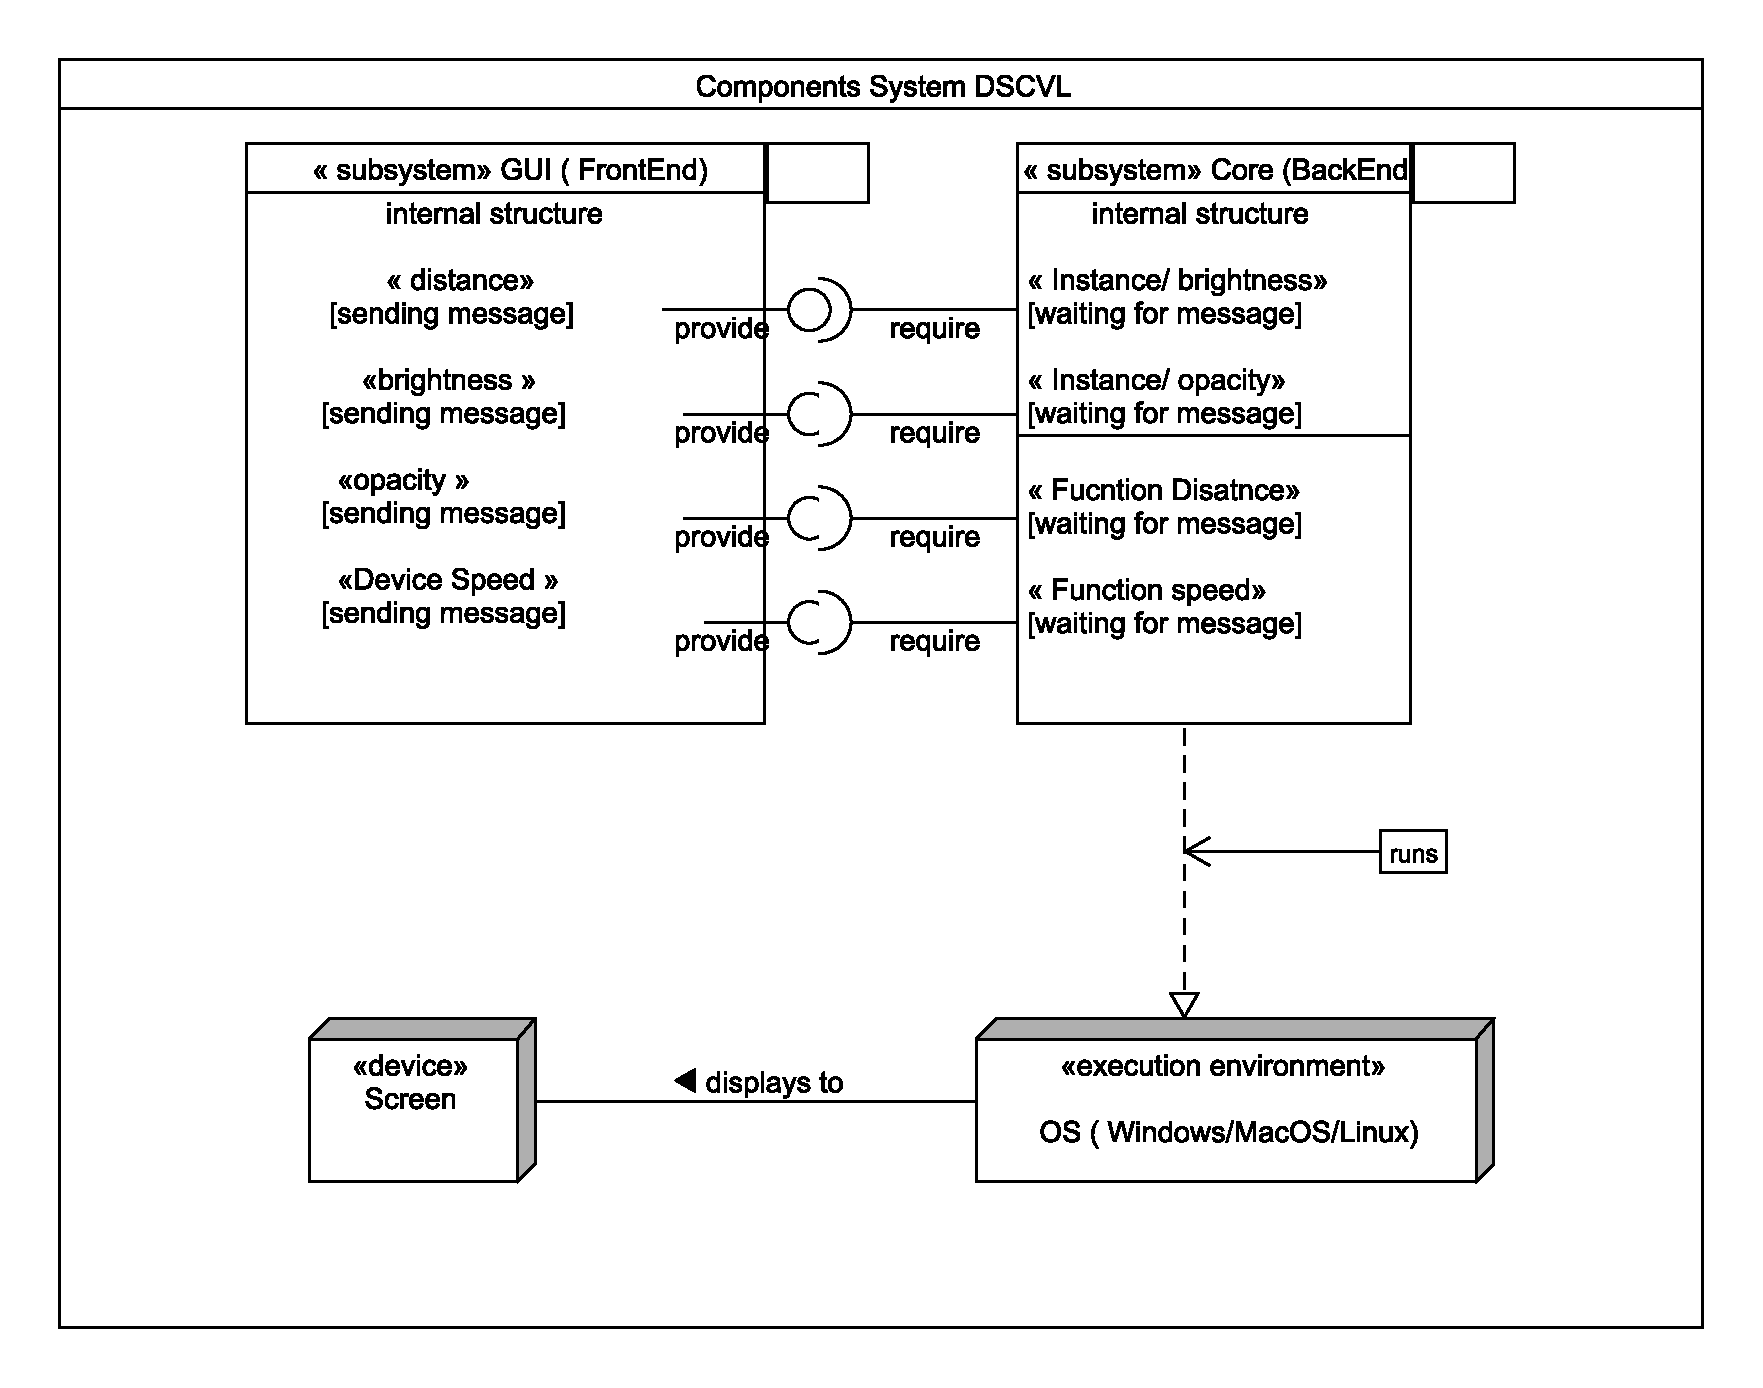
\includegraphics[width=4.5in,natwidth=4000,natheight=200]{images/components.eps}
    	\captionof{figure}{ UML Component diagram for DSCVL} 
    	\end{figure}

		
		\subsubsection{Design Elements}
Other elements of the design are libraries encompassing the almost entire backend. However, this set of libraries is made to be transparent to the user but available to developers. 

      	\subsubsection{Design languages}
   The application to be created would be made in python language though in addition the language, other programming languages  may be added such as the C++ language ( if necessary) in order to run subroutines. Among others, the openCV library plays an important role in the DSCVL software implementation.
   
      \subsubsection{Design Elements - OpenCV and Library Structure}\label{des:LibStructure}
 One sample code functionality of the openCV library implemented in the DSCVL application would look something like this(code hereafter): 
 
 \begin{center}		
\begin{lstlisting}[language=Python] 
from rplidar import RPLidar

PORT_NAME = '/dev/ttyUSB0'


def run(path):
    '''Main function'''
    lidar = RPLidar(PORT_NAME)
    outfile = open(path, 'w')
    try:
        print('Recording measurments... Press Crl+C to stop.')
        for measurment in lidar.iter_measurments():
            line = '\t'.join(str(v) for v in measurment)
            outfile.write(line + '\n')
    except KeyboardInterrupt:
        print('Stoping.')
    lidar.stop()
    lidar.disconnect()
    outfile.close()

if __name__ == '__main__':
    run(sys.argv[1])
\end{lstlisting} 
\end{center}
record\_measurments.py( code lines that capture scanner measurements)[3]
and the above code is a snippet code that also portrays  the internal program structure. Which on module is to capture data from the RPLidar device that has features as described by following figure. 
		\begin{figure}[ht]
		\centering 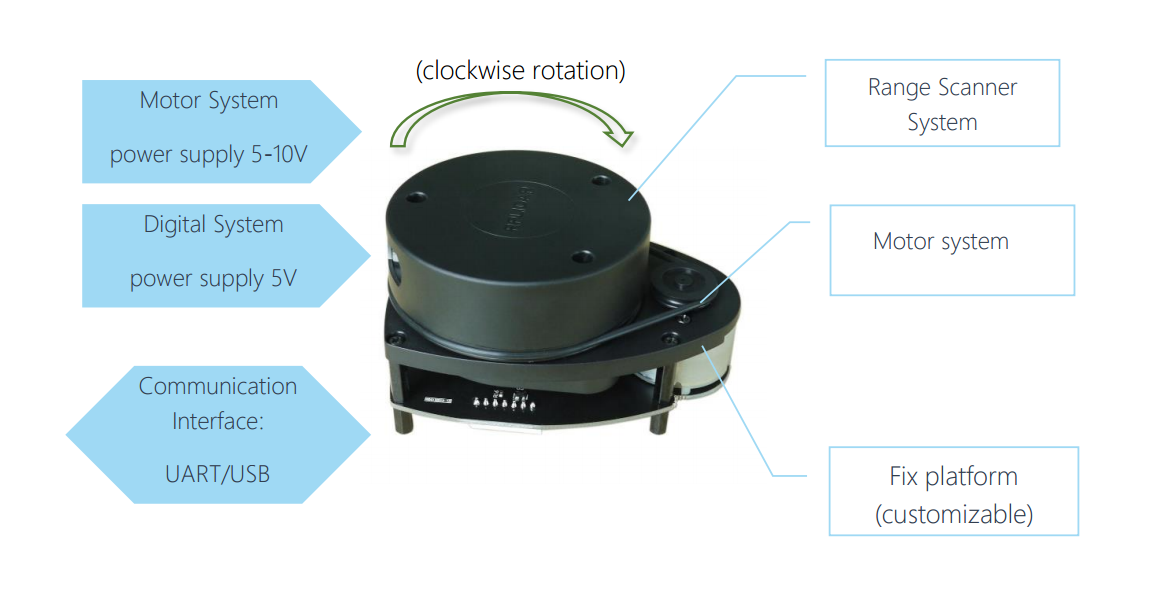
\includegraphics[width=3.5in,natwidth=4000,natheight=400]{images/360rplidar.png}
		
    	 \centering 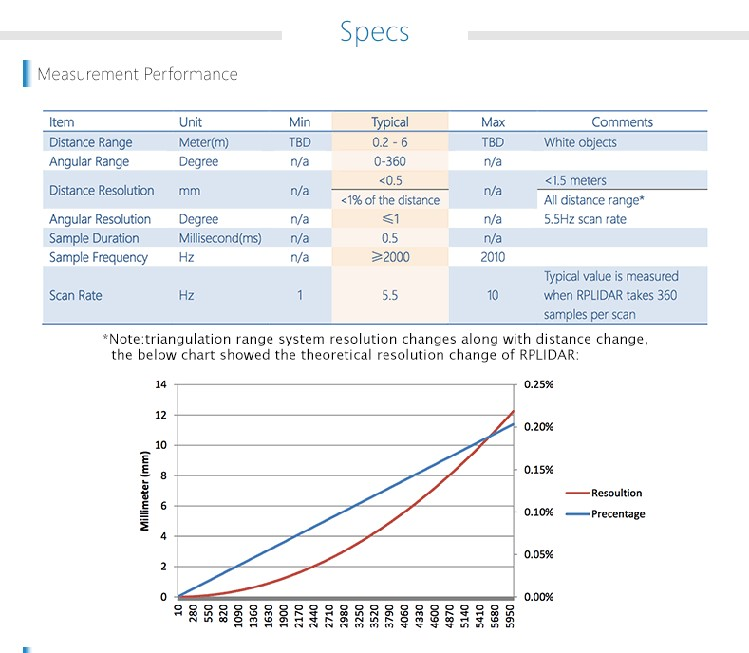
\includegraphics[width=3.5in,natwidth=4000,natheight=400]{images/specifications.jpg}
    	\captionof{figure}{RPLidar device[above]- measurement performance [underneath], derived from \textit{seeeds}} 
    	\end{figure}
\pagebreak
      
      
  
      
  \subsection{Dependency viewpoint and diagram}
  This part is to see how the whole system parts come together as a single entity to perform the require work of getting the overlay image. We have the Interconnection, sharing, and
parameterization of Logitech Brio Webcam and the RPLidar scanner with syncing services happening at the  coding level.

Therefore, we have the following diagram to represent those services.

	\begin{figure}[ht]
			
    \centering 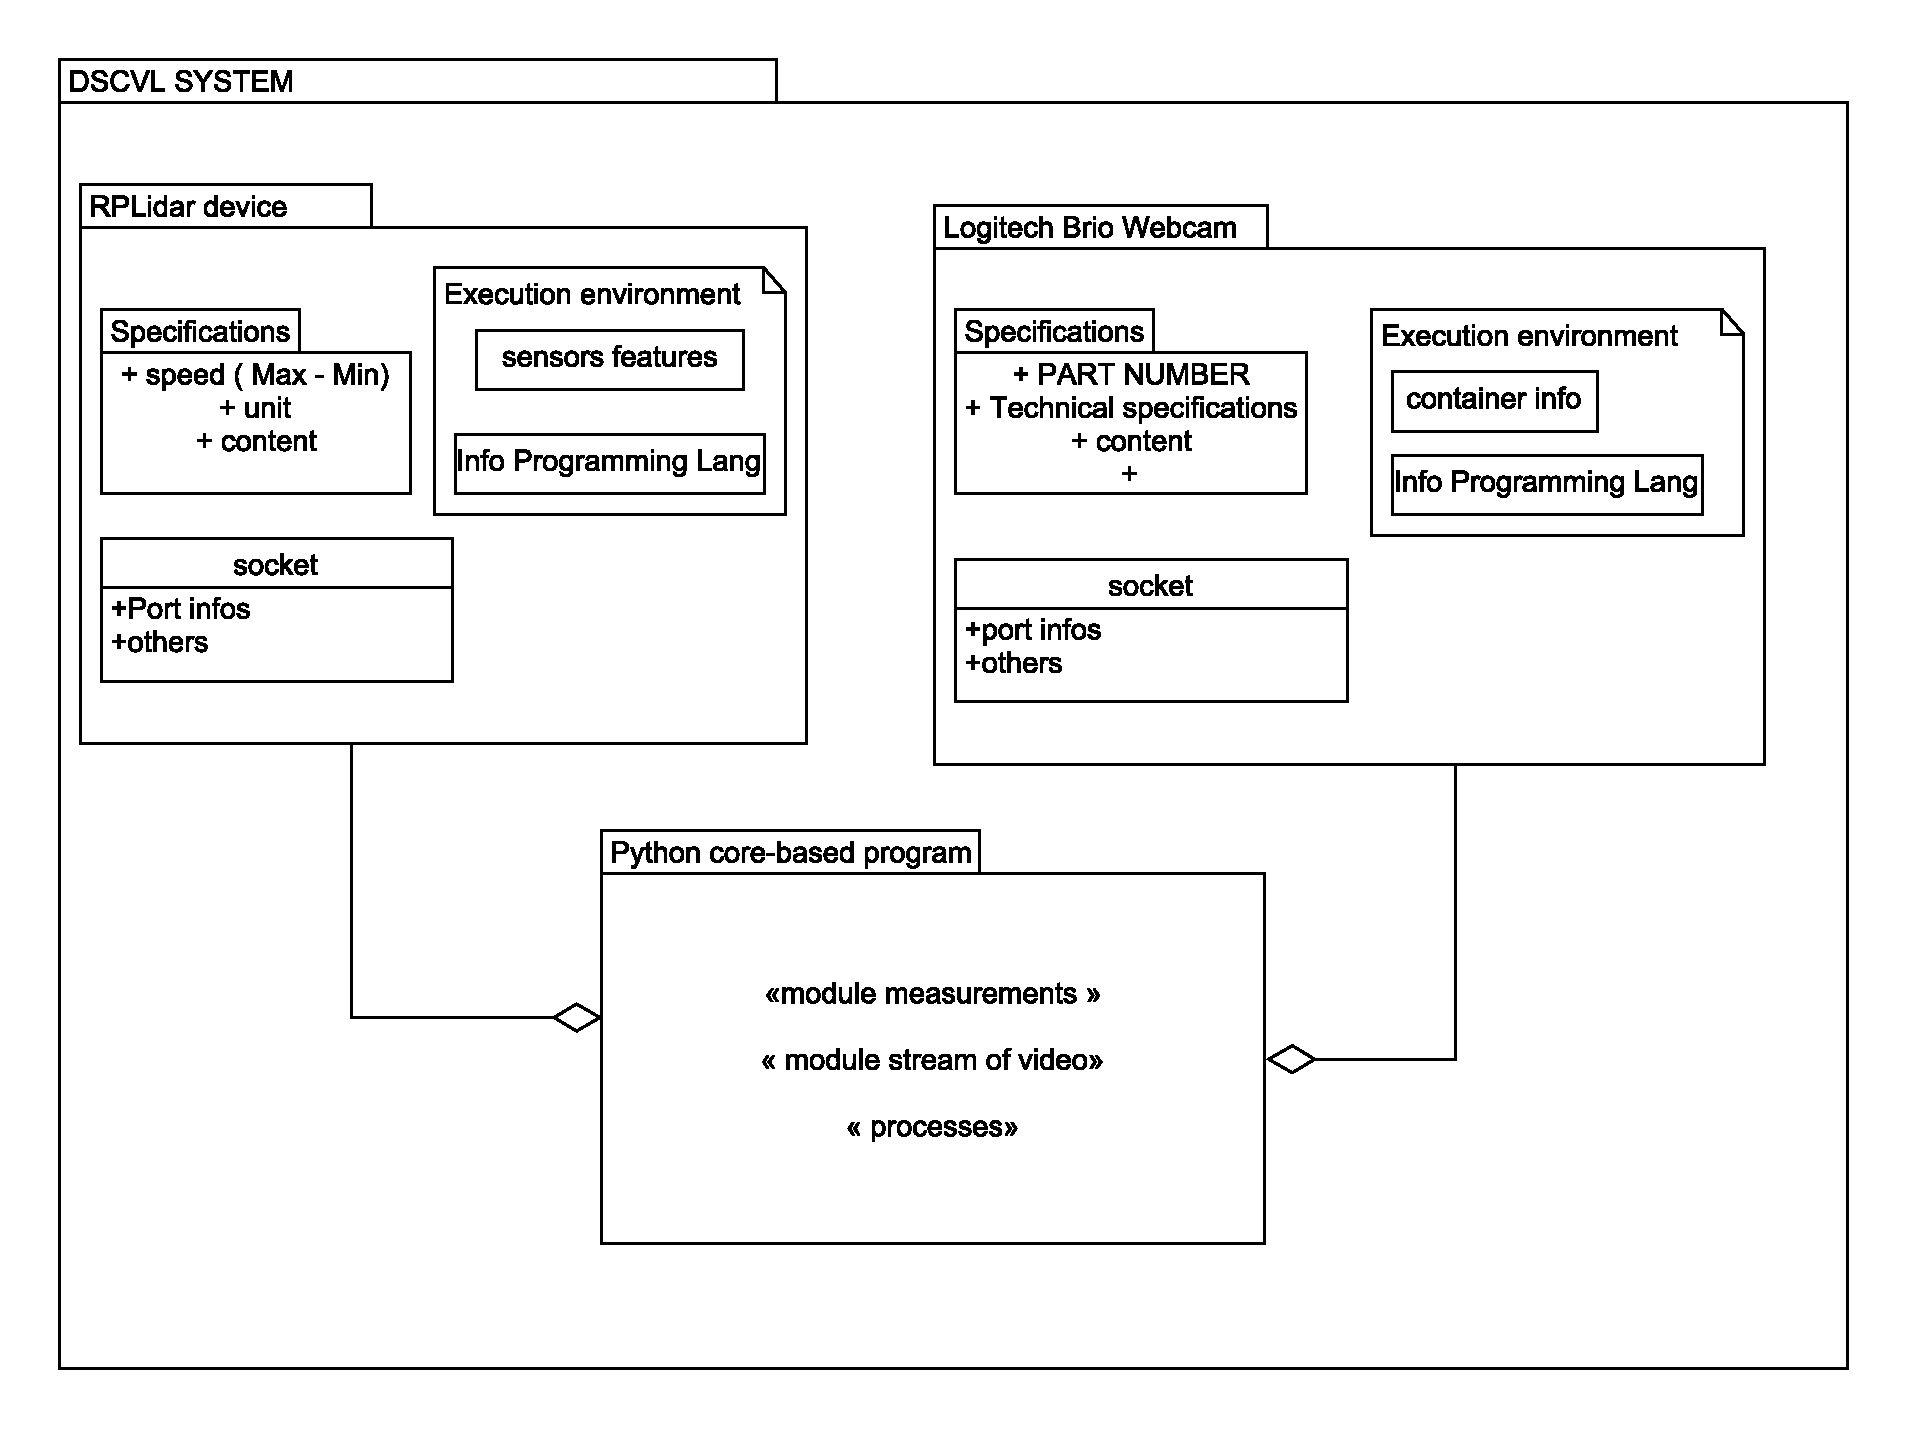
\includegraphics[width=3.5in,natwidth=4000,natheight=400]{images/diagrampackages.eps}
    	\captionof{figure}{ UML package diagram and component diagram} 
    	\end{figure}



      
      \section{References}
[1]: {https://leddartech.com/technology-fundamentals/}   \par	
[2]: {https://www.seeedstudio.com/RPLIDAR-360-degree-Laser-Scanner-Development-Kit-p-1823.html}\par
[3]: {https://github.com/SkoltechRobotics/rplidar/blob/master/examples/record\_measurments.py}
 



\end{document}